\chapter{Gaita Overview} \label{chap:chap-3}


% epigraph after chapter heading
%\epigraph{Since it is written in \LaTeX, it must be true.}{-- Isaac Newton}


%%%% MUST: add the citation for the chapter if it is a reprint

\section{Overview of Design and Purpose}

\subsection{Goals and Objectives}
We introduce Gaita (Generative AI Teaching Assistant) with the primary goal of providing personalized learning pathways out of open access courses for Computer Science learners by leveraging advanced recommendation techniques. Gaita aims to address the challenge of choice overload by offering tailored recommendations that consider learners' background, prior knowledge, and personal goals. By providing more relevant course suggestions, Gaita seeks to enhance learner engagement, improve completion rates, and support users to succeed in their learning journey. Additionally, Gaita supports diverse learners, including those from other fields, by recommending Computer Science courses that are relevant to their specific area of study, ensuring the learning path aligns with their unique goals and background.

\subsection{How Users Interact with Gaita to Generate Recommendations}

Users interact with Gaita through a familiar chatbot interface, where they provide relevant information about their background and learning goals. Upon entering the platform, learners are prompted share details about their current knowledge, experience, and learning objectives (Figure 3.1). 


\begin{figure}[ht]
\begin{center}
    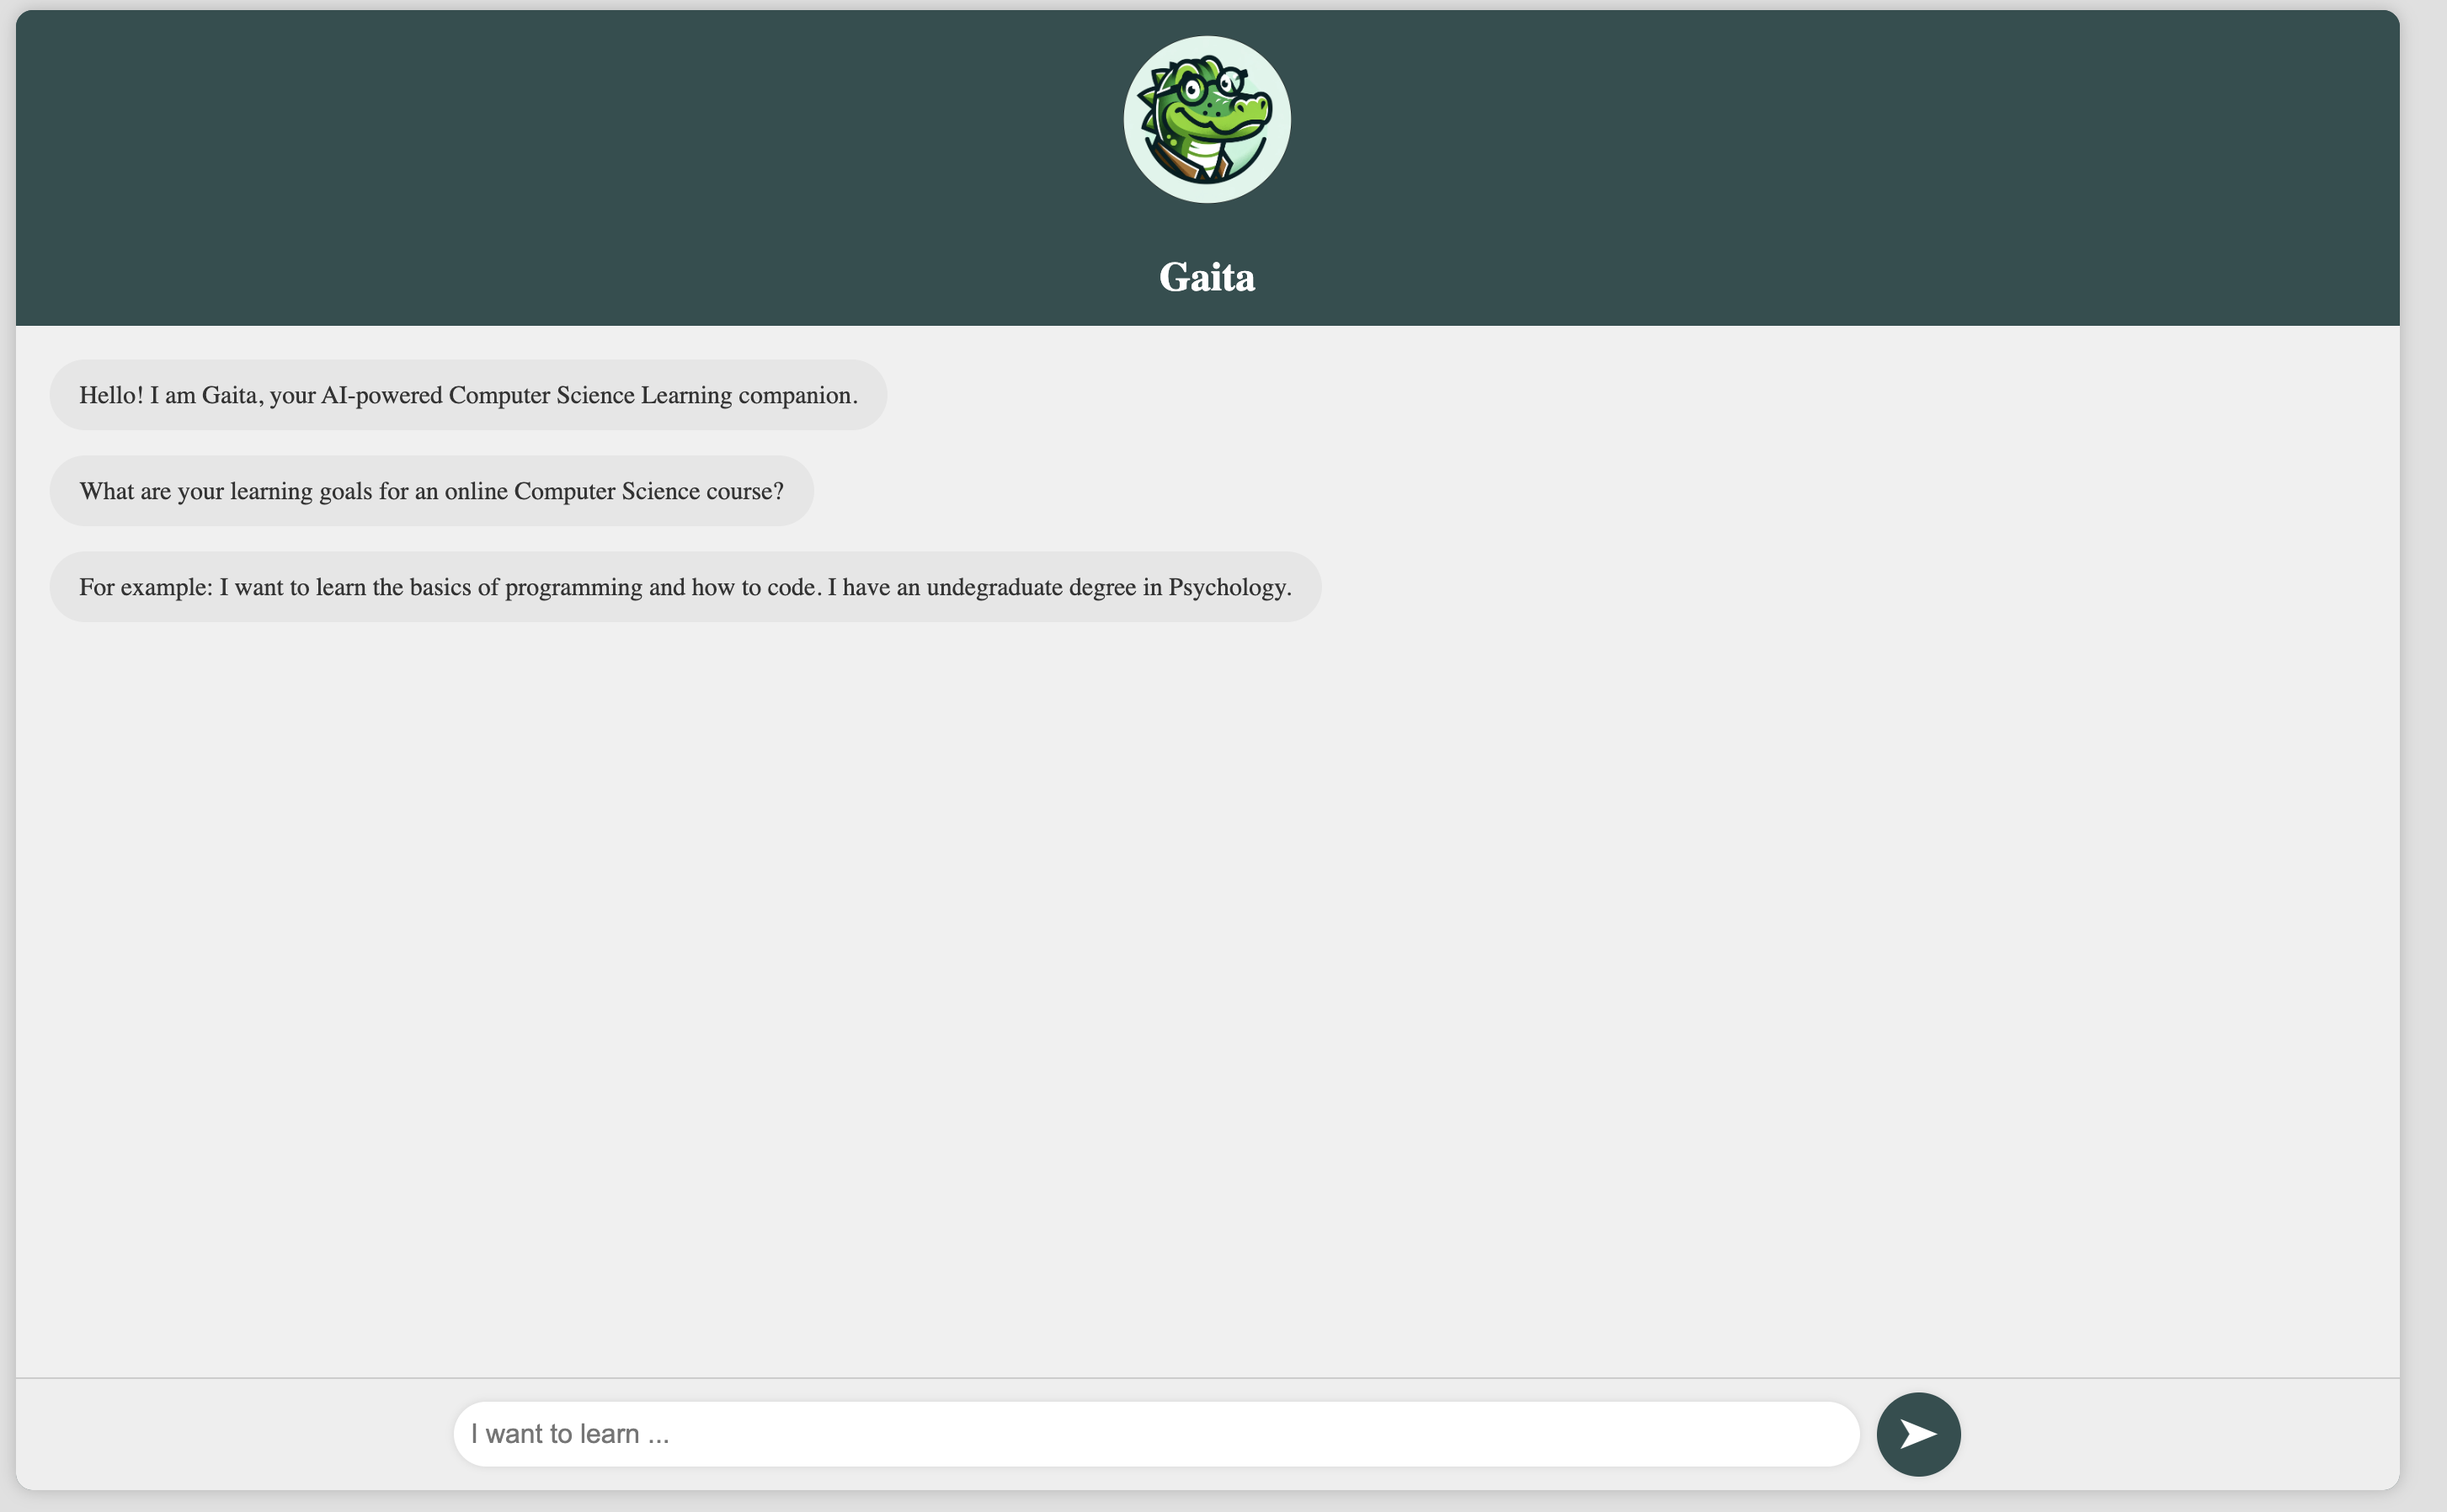
\includegraphics[width=\textwidth] {blankgaita.png}
    \caption{Gaita's Landing Page}
    \label{fig:blankgaita}
\end{center}
\end{figure}


Gaita responds with a list of relevant courses from its RAG database of open-access CS courses, along with descriptions of how they align with the user’s prompt and relevant follow-up questions to assess the learner's experience with prerequisites for the recommended courses, which is where the iterative prompting comes into play. Based on the user's responses, Gaita suggests appropriate prerequisite courses to bridge any knowledge gaps (Figure 3.2.1).

\begin{figure}
    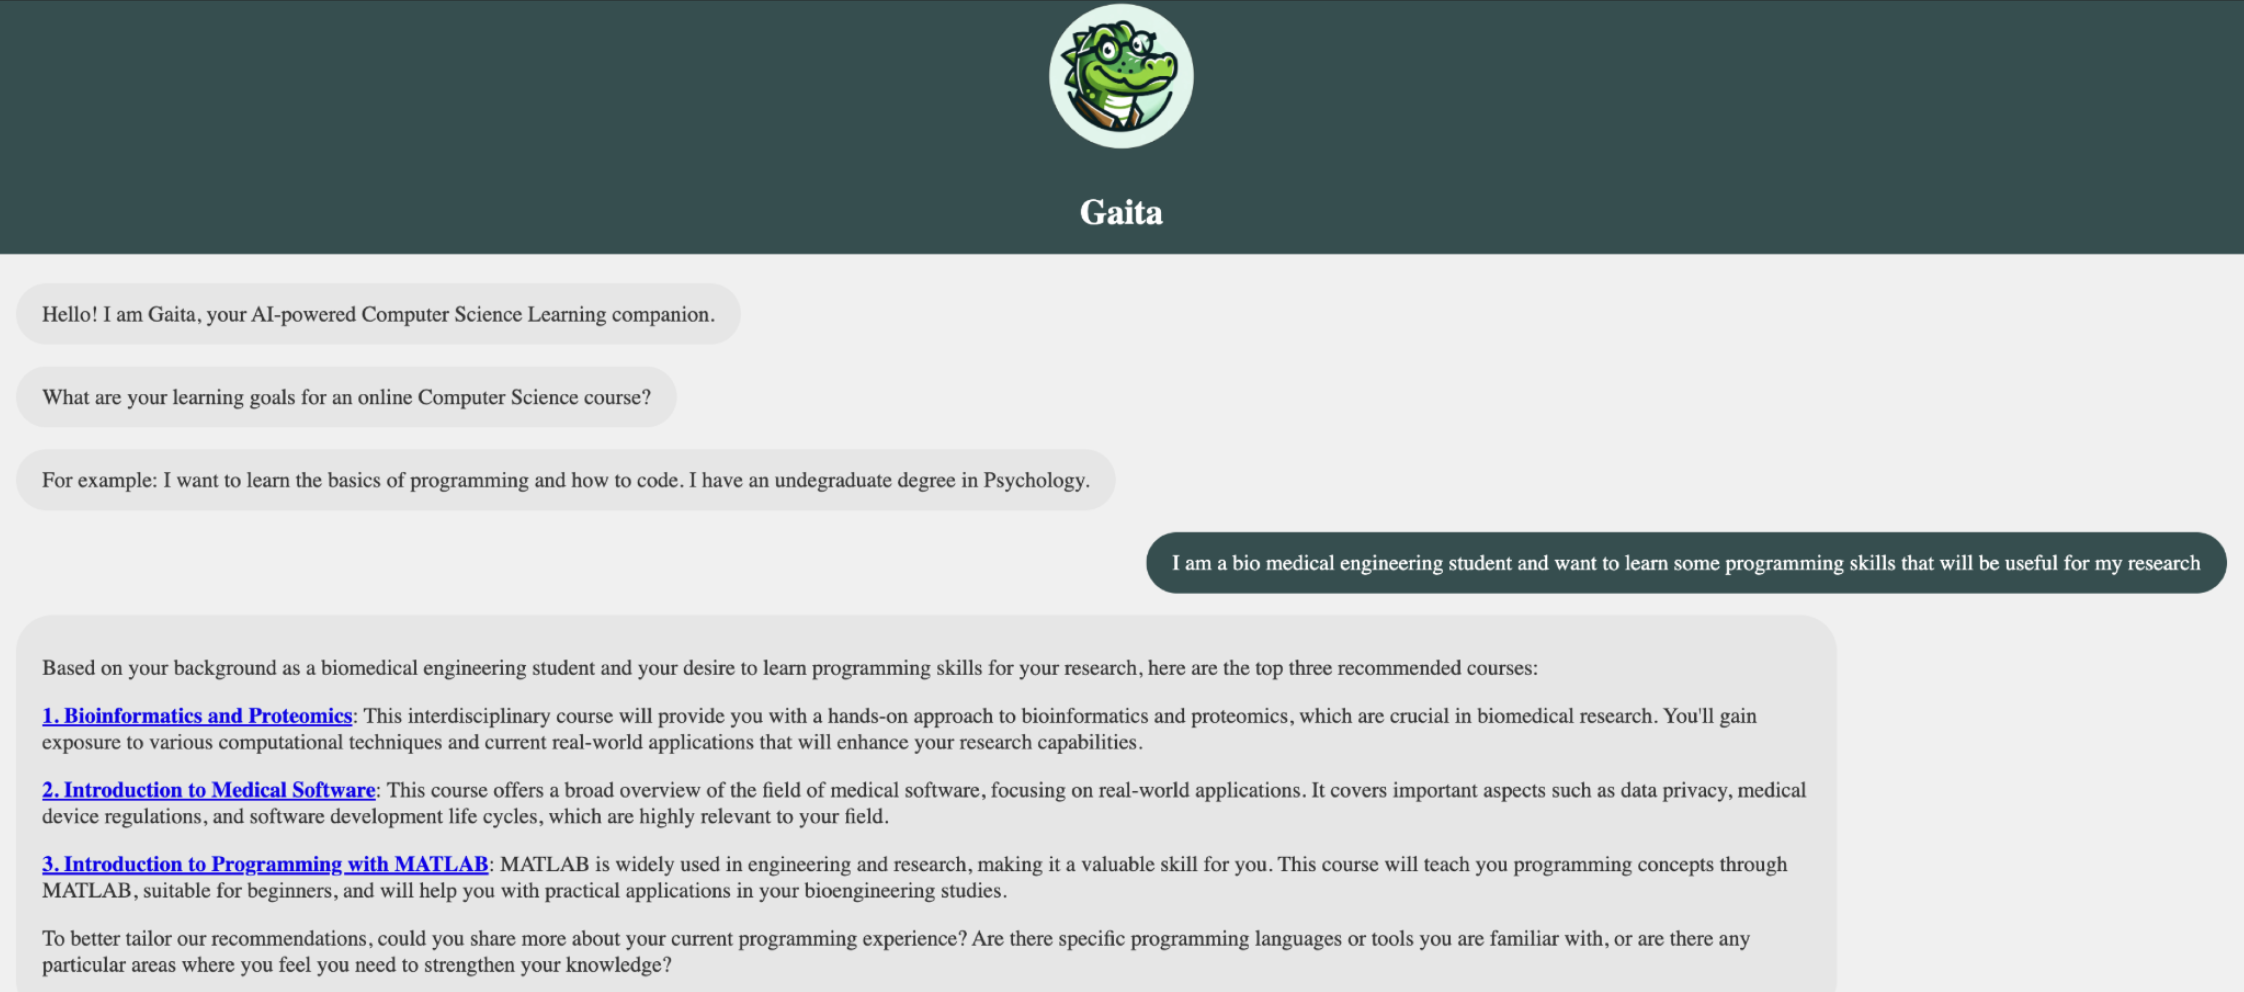
\includegraphics[width=1\linewidth]{figures/ex1a.png}
    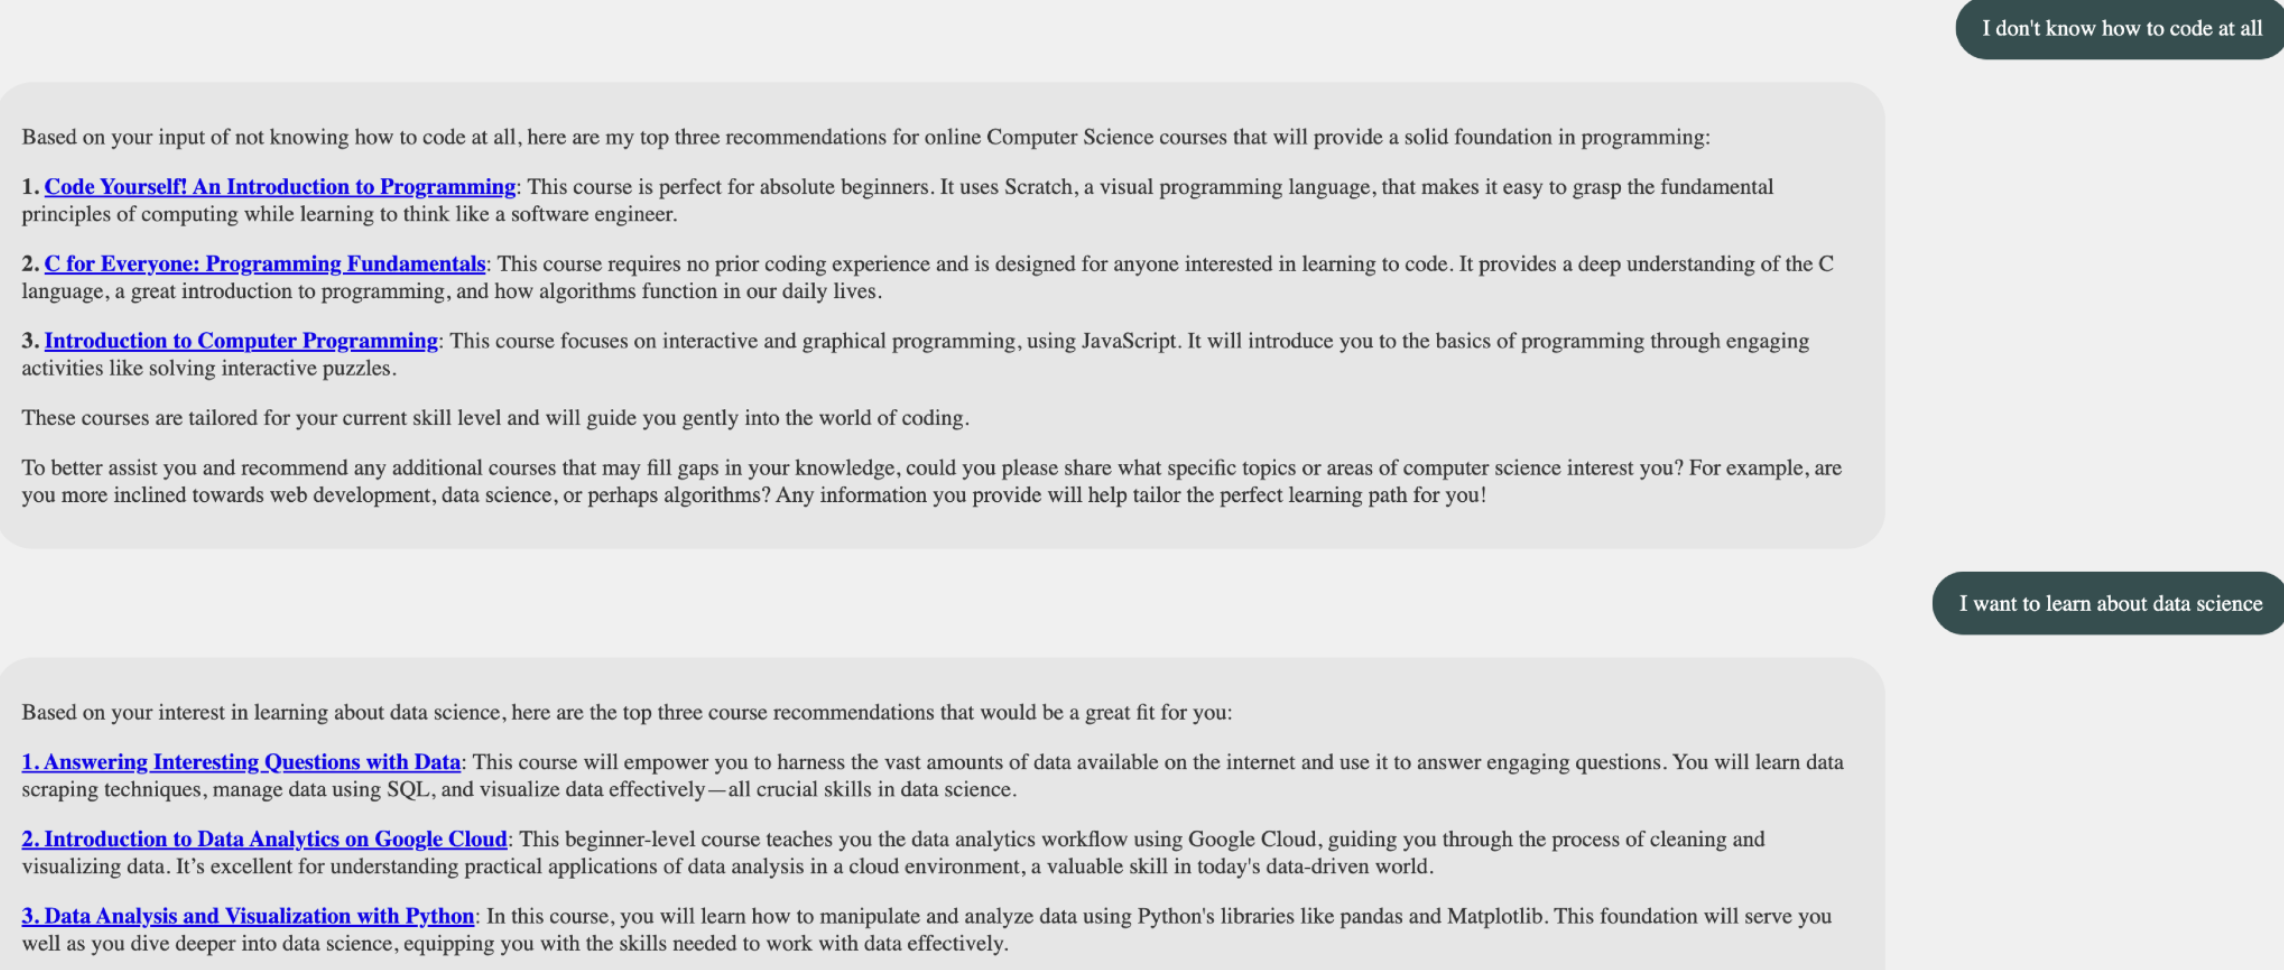
\includegraphics[width=1\linewidth]{figures/ex1b.png}
    \caption{Sample Interaction}
    \label{fig:hu}
\end{figure}



The system iteratively refines its suggestions based on the learner's feedback, which ensures that the learning path remains relevant and aligned with the learner's evolving needs (Figure 3.2.2).


\subsection{How Learners' Background and Goals Influence their Learning Path}

The input provided by learners—such as their background, previous experience, and specific learning goals—directly shapes the learning paths generated by Gaita. For example, learners with a background in a different field or those transitioning into Computer Science will receive recommendations for foundational courses that address gaps in their knowledge. Meanwhile, learners with prior experience in certain areas will be guided toward more advanced or specialized content. By considering these inputs, Gaita ensures that the recommendations are not only relevant but also adaptable to each learner's prior knowledge.

\section{Justification for Components} 
For the components chosen in Gaita, the decision to implement a chatbot interface was driven by the goal of enabling an interactive, iterative recommendation process that allows users to discover learning pathways tailored to their experience. The chatbot allows learners to input natural language prompts where they can detail their prior experience, share their goals, and build their course pathway throughout the conversation. This approach enables a more natural, adaptive experience compared to traditional forms of search. 

Starting with learners' goals is a key component of the system's design. By focusing on their objectives from the outset, Gaita is able to generate more relevant and targeted course recommendations. Additionally, the system generates follow-up questions regarding user comfort with the prerequisites to help bridge any knowledge gaps with additional recommendations. Working backwards from the user’s goals to bridge knowledge gaps ensures that the user does not take irrelevant introductory courses. 

We chose to restrict the recommendations to courses from Coursera and MIT OpenCourseWare because both platforms are well-known and trusted, offering courses from reputable institutions. These platforms are widely recognized in the education space, and their courses are regularly updated and highly relevant, making them ideal sources for the initial course database. While centralizing CS resources is important, the primary focus of this project is on the recommendation pipeline and creating a personalized learning experience, rather than the data collection process itself. Our current database contains over 1,200 courses, and the modular nature of our system allows additional courses and platforms to be added in the future with minimal difficulty. 

Although collaborative filtering using additional user data is a possibility, we decided not to scrape course reviews or LinkedIn data at this stage, as both are outside the scope of this project. While user reviews could provide valuable insights, they would introduce challenges related to data quality, filtering, and other ethical considerations. Similarly, scraping LinkedIn profiles raises privacy concerns and adds complexity, making it more appropriate for future iterations of the system if necessary.

\section{Data Sources}

Gaita uses open-access Computer Science courseware from Coursera and MIT OpenCourseWare, which provide high-quality courses from well-known institutions. These sources were chosen for their credibility and extensive offerings. The current database includes over 1,200 courses, collected via web crawling to efficiently aggregate up-to-date course data. 

%\blindtext\footnote{Hello, this is the first footnote with no indentation and single-spaced text. The spacing between two footnotes is also single-spaced.}